\documentclass[12pt,a4paper]{article}
\usepackage{amsmath,amssymb,tikz,mathrsfs,tkz-tab}
\usepackage[top=1cm, bottom=1.5cm, left=1.5cm, right=1.5cm]{geometry}
\usepackage[color]{ex_test} % color, loigiai, solcolor, book
\renewcommand{\baselinestretch}{1.5}
\begin{document}
\begin{center}
\textbf{\LARGE ĐỀ MINH HỌA}
\end{center}
\subsection*{PHẦN I. Câu trắc nghiệm nhiều phương án lựa chọn. Thí sinh trả lời từ câu 1 đến câu 12. Mỗi câu hỏi thí sinh chỉ chọn một phương án.}
	\setcounter{ex}{0}
	\Opensolutionfile{ans}[ans/ans-phanI]
\begin{ex}
Mệnh đề toán học nào sau đây là mệnh đề sai?
\choice
{Số 2 là số nguyên}
{Số 2 là số hữu tỉ}
{Số 2 là số hữu ti dương}
{\True Số 2 không là số nguyên tố}
\loigiai
{

}
\end{ex}
\begin{ex}
Cho hai tập hợp $A$ và $B$. Tập hợp $A \cap B$ là
\choice
{tập hợp tất cả các phần tử thuộc $A$ hoặc thuộc $B$}
{\True tập hợp tất cả các phần tử vừa thuộc $A$ vừa thuộc $B$}
{tập hợp các phần tử thuộc $A$ nhưng không thuộc $B$}
{tập hợp tất cả các phần tử thuộc $B$ nhưng không thuộc $A$}
\loigiai
{

}
\end{ex}
\begin{ex}
Tập hợp rỗng là
\choice
{tập hợp có đúng 1 phần tử}
{tập hợp có đúng 2 phần từ}
{tập hợp có vô số phần tử}
{\True tập hợp không có phần tử nào}
\loigiai
{

}
\end{ex}
\begin{ex}
Cho hai tập hợp $A$ và $B$ khác $\varnothing$. Tập hợp $A$ là tập hợp con của tập hợp $B$ khi và chỉ khi
\choice
{có một phần tử của $A$ là phần tử của $B$}
{mọi phần tử của $B$ đều là phần tử của $A$}
{\True mọi phần tử của $A$ đều là phần tử của $B$}
{hiệu của $A$ và $B$ là tập hợp khác rỗng}
\loigiai
{

}
\end{ex}
\begin{ex}
Phát biểu nào nào sau đây là đúng?
\choice
{\True Với hai vectơ bất kì $\vec{a}, \vec{b}$ và số thực $k$, ta có: $k(\vec{a}+\vec{b})=k \vec{a}+k \vec{b}$}
{Với hai vectơ bất ki $\vec{a}, \vec{b}$ và số thực $k$, ta có: $k(\vec{a}+\vec{b})=\vec{a} k+\vec{b} k$}
{Với hai vectơ bất kì $\vec{a}, \vec{b}$ và số thực $k$, ta có: $(\vec{a}+\vec{b}) k=\vec{a} k+\vec{b} k$}
{Với hai vectơ bất kì $\vec{a}, \vec{b}$ và số thực $k$, ta có: $k(\vec{a}+\vec{b})=k \vec{a}+\vec{b} k$}
\loigiai
{

}
\end{ex}
\begin{ex}
Cho góc nhọn $\alpha$ tùy ý. Phát biểu nào sau đây là đúng?
\choice
{\True $\sin (90-\alpha)=\cos \alpha$}
{$\sin (90-\alpha)=\sin \alpha$}
{$\sin (90-\alpha)=-\sin \alpha$}
{$\sin (90-\alpha)=-\cos \alpha$}
\loigiai
{

}
\end{ex}

\begin{ex}
Cho góc nhọn $\alpha$ tùy ý. Phát biểu nào sau đây là đúng?
\choice
{$\cos (180-\alpha)=\cos \alpha$}
{$\cos (180-\alpha)=\sin \alpha$}
{\True $\cos (180-\alpha)=-\cos \alpha$}
{$\cos (180-\alpha)=-\sin \alpha$}
\loigiai
{

}
\end{ex}
\begin{ex}
Cho $G$ là trọng tâm $\triangle A B C$ và điểm $M$ tùy ý. Phát biểu nào sau đây là đúng?
\choice
{$\overrightarrow{M A}+\overrightarrow{M B}+\overrightarrow{M C}=\overrightarrow{0}$}
{$\overrightarrow{M A}+\overrightarrow{M B}+\overrightarrow{M C}=\overrightarrow{M G}$}
{$\overrightarrow{M A}+\overrightarrow{M B}+\overrightarrow{M C}=2 \overrightarrow{M G}$}
{\True $\overrightarrow{M A}+\overrightarrow{M B}+\overrightarrow{M C}=3 \overrightarrow{M G}$}
\loigiai
{

}
\end{ex}
\begin{ex}
Cho tam giác nhọn $A B C$ nội tiếp đường tròn bán kính $R$. Phát biểu nào sau đây là đúng?
\choice
{\True $\dfrac{B C}{\sin A}=2 R$}
{$\dfrac{B C}{\cos A}=2 R$}
{$\dfrac{A B}{\cos A}=2 R$}
{$\dfrac{A B}{\sin A}=2 R$}
\loigiai
{

}
\end{ex}
\begin{ex}
Cho tam giác $A B C$. Phát biểu nào sau đây là đúng?
\choice
{\True $B C^2=A B^2+A C^2+2 A B \cdot A C \cdot \cos A$}
{$B C^2=A B^2+A C^2-2 A B \cdot A C \cdot \cos A$}
{ $B C^2=A B^2+A C^2+2 A B \cdot A C \cdot \sin A$}
{$B C^2=A B^2+A C^2-2 A B \cdot A C \cdot \sin A$}
\loigiai
{

}
\end{ex}
\begin{ex}
Cho đoạn thẳng $A B$ và hai điểm $M, N$ thuộc đoạn thẳng $A B$ sao cho: $2 M A=3 M B$. Phát biểu nào sau đây là đúng?
\choice
{ $2 \overrightarrow{M A}=3 \overrightarrow{M B}$}
{\True $2 \overrightarrow{M A}=-3 \overrightarrow{M B}$}
{$2 \overrightarrow{A B}=3 \overrightarrow{A M}$}
{$3 \overrightarrow{B M}=\overrightarrow{B A}$}
\loigiai
{

}
\end{ex}
\begin{ex}
\immini
{
Cho hệ bất phương trình bậc nhất hai ẩn
$$
\left\{\begin{array}{l}
x-y \geq 0 \\
x-y \leq 2 \\
x+y \geq 0 \\
x+y \leq 4
\end{array}\right.
$$
có miền nghiệm được biểu diễn là hình tứ giác $O A B C$ (tham khảo hình vẽ).
Giá trị lớn nhất của biểu thức $L=2 x+y$ bằng bao nhiêu?
}
{
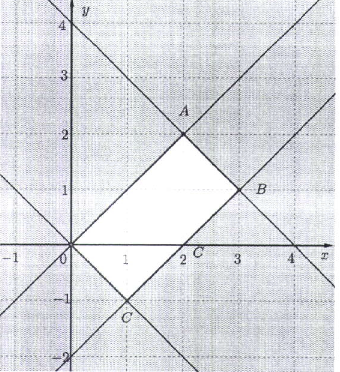
\includegraphics[scale=0.8]{images/imMH-1}
}
\choice
{ 6}
{\True 7}
{8}
{5}
\loigiai
{
}
\end{ex}

	\Closesolutionfile{ans}

\subsection*{PHẦN II. Câu trắc nghiệm đúng sai. Thí sinh trả lời từ câu 1 đến câu 4. Trong mỗi ý a), b), c), d) ở mỗi câu, thí sinh chọn đúng hoặc sai.}
	\setcounter{ex}{0}
	\Opensolutionfile{ans}[ans/ans-phanII]
\begin{ex}
Một cuộc thi bắn cung có 20 người tham gia. Trong lần bắn đầu tiên có 18 người bắn trúng mục tiêu. Trong lần bắn thứ hai có 15 người bắn trúng mục tiêu. Trong lần bắn thứ ba chỉ còn 10 người bắn trúng mục tiêu.
\choiceTF
{\True Số người bắn trượt mục tiêu trong lần đầu tiên là 2}
{Số người bắn trượt mục tiêu trong lần bắn thứ hai là 6}
{Số người bắn trượt mục tiêu trong lần bắn thứ nhất và thử hai nhiều nhất là 8}
{\True Số người bắn trúng mục tiêu trong cả ba lần bắn ít nhất là 3}
\loigiai
{
}
\end{ex}
\begin{ex}
Cho tứ giác $A B C D$ có $M, N$ lần lượt là trung điểm của các cạnh $A B, C D$. Gọi $O$ là trung điểm của đoạn thẳng $M N$ và $G$ là trọng tâm tam giác $A B C$.
\choiceTF
{\True $\overrightarrow{D A}+\overrightarrow{D B}=2 \overrightarrow{D M}$}
{$\overrightarrow{D A}+\overrightarrow{D B}+\overrightarrow{D C}=2 \overrightarrow{D O}$}
{$\overrightarrow{D A}+\overrightarrow{D B}+\overrightarrow{D C}=2 \overrightarrow{D G}$}
{$\overrightarrow{D O}=2 \overrightarrow{D G}$}
\loigiai
{

}
\end{ex}
\begin{ex}
\immini
{
Cho hình bình hành $A B C D$. Gọi $O$ là giao điểm của $A C$ và $B D$ (Hình bên).
\choiceTF
{\True $\overrightarrow{O A}$ và $\overrightarrow{O C}$ là hai vectơ dối nhau}
{$\overrightarrow{O B}$ và $\overrightarrow{D O}$ là hai vectơ đối nhau}
{\True $\overrightarrow{O A}+\overrightarrow{O C}=\overrightarrow{O B}+\overrightarrow{O D}$}
{\True $\overrightarrow{O A}+\overrightarrow{O B}+\overrightarrow{O C}+\overrightarrow{O D}=\overrightarrow{A D}+\overrightarrow{C B}$}
}
{
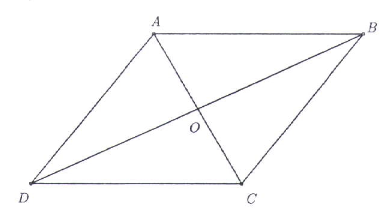
\includegraphics[scale=1]{images/imMH-3}
}
\loigiai
{

}
\end{ex}
\begin{ex}
Lớp $10 ~A$ có 40 học sinh, trong đó có 27 học sinh tham gia câu lạc bộ bóng rồ và 25 học sinh tham gia câu lạc bộ bóng đá.
\choiceTF
{\True Số học sinh tham gia câu lạc bộ bóng rổ hoặc tham gia câu lạc bộ bóng đá nhiều nhất là 40}
{Số học sinh tham gia cả hai câu lạc bộ bóng rổ và bóng đá ít nhất là 10}
{Số học sinh không tham gia cả hai câu lạc bộ bóng rổ và bóng đá ít nhất là 1}
{Số học sinh không tham gia cả hai câu lạc bộ bóng rổ và bóng đá nhiều nhất là 10}
\loigiai
{

}
\end{ex}

	\Closesolutionfile{ans}

\subsection*{PHẦN III. Câu trắc nghiệm trả lời ngắn. Thí sinh trả lời từ câu 1 đến câu 6.}
	\setcounter{ex}{0}
	\Opensolutionfile{ans}[ans/ans-phanIII]
\begin{ex}
Cho hình chữ nhật $A B C D$ có $A B=4, A D=6$. Độ dài của vectơ $\vec{u}=\overrightarrow{A B}+\overrightarrow{A C}$ bằng bao nhiêu?
\shortans{$10$}
\end{ex}
\begin{ex}
\immini
{
Để đo khoảng cách từ vị trí $A$ đến vị trí $B$ ở hai bên bờ hồ, bạn Hà tiến hành đo khoảng cách $A C$ và các góc $\widehat{B A C}, \widehat{B C A}$. Kết quả nhận được là: $A C=21 ~m, \widehat{B A C}=58^{\circ}$ và $\widehat{B C A}=80^{\circ}$ (Hình bên). Khoảng cách từ vị trí $A$ đến vị trí $B$ là bao nhiêu mét (làm tròn kết quả đến hàng đơn vị của mét)?
}
{
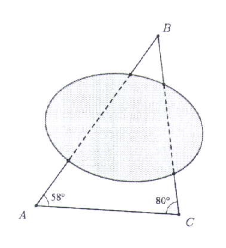
\includegraphics[scale=0.7]{images/imMH-2}
}
\shortans{$31$}
\end{ex}
\begin{ex}
Hai tàu đánh cá cùng xuất phát từ bến $A$ và đi về hai vùng biển khác nhau theo hai nửa đường thẳng tạo với nhau một góc $60^{\circ}$. Tàu thứ nhất chạy với tốc độ 8 hải lí một giờ và tàu thứ hai chạy với tốc độ 12 hải lí một giờ. Sau đúng 2 giờ thì khoảng cách giữa hai tàu là bao nhiêu hải lí (làm tròn kết quả đến hàng đơn vị của hải lí)?
\shortans{$21$}
\end{ex}
\begin{ex}
Có 100 tấm thẻ được đánh số thứ tự từ 1 đến 100 và được đặt ngửa trên bàn. Người ta lật ngược các tấm thẻ như sau:
Lần thứ nhất, lật ngược tất cả các tấm thẻ có số thứ tự chia hết cho 2.
Lần thứ hai, lật ngược tất cả các tấm thẻ có số thứ tự chia hết cho 5.
Hỏi sau lần thứ hai, có bao nhiêu tấm thẻ được đặt sấp. Biết rằng, khi bị lật ngược, thẻ đang ngửa sẽ thành sấp và thẻ đang sấp sẽ thành ngửa.
\shortans{$50$}
\end{ex}
\begin{ex}
Để chế biến một hộp thực phẩm $A$ cần $0,2 ~kg$ cà chua và $0,1 ~kg$ thịt; một hộp thực phẩm $B$ cần $0,2 ~kg$ cà chua và $0,3 ~kg$ thịt. Lợi nhuận thu được từ 1 hộp thực phầm $A$ và 1 hộp thực phẩm $B$ lần lượt là 4000 đồng và 5000 đồng. Chị Hoa có $2 ~kg$ cà chua và $2 ~kg$ thịt để sản xuất các hộp thực phẩm $A$ và $B$. Với lượng nguyên liệu như trên, lợi nhuận lớn nhất chị Hoa có thể thu được là bao nhiêu nghìn đồng?
\shortans{$45$}
\end{ex}
\begin{ex}
Một xưởng sản xuất bàn và ghế. Thời gian để một công nhân hoàn thiện 1 chiếc bàn và 1 chiếc ghế lần lượt là 120 phút và 30 phút. Xưởng có 4 công nhân, mỗi công nhân làm việc không quá 6 tiếng mỗi ngày. Biết rằng sản phẩm của xưởng luôn được tiêu thụ hết, mỗi chiếc bàn lãi 200 nghìn đồng, mỗi chiếc ghế lãi 75 nghìn đồng và số ghế không vượt quá 4 lần số bàn. Trong một ngày sản xuất, xưởng có thể thu được lợi nhuận lớn nhất là bao nhiêu tiền? Viết câu trả lời theo đơn vị triệu đồng.
\shortans{$3$}
\end{ex}
\Closesolutionfile{ans}
	
%%=====================
\begin{center}
\textbf{\large BẢNG ĐÁP ÁN}
\end{center}
\noindent\textbf{A. ĐÁP ÁN PHẦN I}
\inputansbox{10}{ans/ans-phanI}
	
\noindent\textbf{B. ĐÁP ÁN PHẦN II}
\inputansbox[5]{5}{ans/ans-phanII}
	
\noindent\textbf{C. ĐÁP ÁN PHẦN III}
\inputansbox[3]{6}{ans/ans-phanIII}
\end{document}

